\documentclass[letterpaper, 10 pt, conference]{ieeeconf} % letterpaper/a4paper 
% ieeeconf IEEEtran
\IEEEoverridecommandlockouts   % Needed if you want to use the \thanks command
\overrideIEEEmargins

\usepackage{amsmath} 
\usepackage{graphicx}
\usepackage[ruled,vlined]{algorithm2e}
\usepackage{amsfonts} % for mathbf and mathbb
\usepackage{hyperref} % required because bib generates \url{}
\usepackage{verbatim} % For begin{comment} end{comment}
\usepackage{authblk} % useful for multiple authors with different affiliations
\usepackage{cite} % useful to show multiple citations in single square bracket
\usepackage{subfig}
\providecommand{\DontPrintSemicolon}{\dontprintsemicolon} % difference in versions

\DeclareMathOperator*{\argmin}{arg\,min}
\DeclareMathOperator*{\argmax}{arg\,max}
\newcommand{\vect}[1]{\mathbf{#1}}
\newcommand{\hvect}[1]{\bar{\vect{#1}}}
\newcommand{\uvect}[1]{\hat{\vect{#1}}}
\newcommand{\field}[1]{\mathbb{#1}}
\newcommand{\Real}[0]{\field{R}}


\title{\Large \bf
Modern MAP inference methods for accurate and faster occupancy grid mapping on higher
order factor graphs
}
\author[1]{Vikas Dhiman}
\author[2]{Abhijit Kundu}
\author[2]{Frank Dellaert}
\author[1]{Jason J. Corso}
\affil[1]{ Department of Computer Science and Engineering, SUNY at Buffalo, NY, USA }
\affil[1]{{\tt\small\{vikasdhi,jcorso\}@buffalo.edu}}
\affil[2]{College of Computing, Georgia Tech, GA, USA}
\affil[2]{{\tt\small\{abhijit.kundu,frank\}@gatech.edu}}

\begin{document}
\maketitle
\begin{abstract}
Using the inverse sensor model has been popular in occupancy grid mapping. 
However, it is widely known that applying the inverse sensor model to mapping 
requires certain assumptions that are not necessarily true. Even work that uses 
forward sensor models have relied on methods like expectation maximization or 
Gibbs sampling which have been succeeded by more effective methods of maximum a 
posteriori (MAP) inference over graphical models. In this paper, we propose the 
use of modern MAP inference methods along with the forward sensor model.  Our 
implementation and experimental results demonstrate that these modern inference 
methods deliver more accurate maps more efficiently than previously used 
methods.
\end{abstract}
\section{Introduction}
% % Outline
% * [X] Describe the problem. How it is important for robotics?
% * [X] What are different ways of solving problem?
% * [X] Do we focus on a particular way of solving?
% * [X] What is the common trend?
% * [X] What is wrong  with current approach?
% * [X] What are we proposing?
% * [X] Has someone done this before? If yes, how are we different.

Mobile robot problems like navigation, path planning, localization and collision 
avoidance require an estimate of the robot's spatial environment; this 
underlying problem is called robot mapping\cite{thrun2002robotic}.  Even in 
environments where maps are available, the environment may change over time 
necessitating a mapping ability on the mobile robot.  Robot mapping hence 
remains an active field of research 
\cite{meyer2012occupancy,nagla2012improved,merali2013icra} as it is an important 
problem in application areas like indoor autonomous navigation, grasping, 
reconstruction and augmented reality.

% This paragraph just provides some information that should be widely known; I'm 
% not sure it should be included.  At the least, it can be removed if space is 
% an issue.
Although robot mapping can be performed in a many ways---metric or topological; 
with range sensors, like sonar \cite{thrun2003learning}, laser scanners 
\cite{thrun2003learning} and RGBD \cite{newcombe2011kinectfusion}, or 
bearing-only sensors \cite{davison2007monoslam,kundu2011realtime}---metric 
mapping with range sensors is the most common.  Bearing-only sensors provide 
estimates up to a scale factor; topological maps still require local metric 
estimates for certain problems like navigation.  We hence focus on metric 
mapping with range sensors, specifically, laser scanners.

Occupancy grid mapping (OGM) is a popular and useful range-based mapping methods 
\cite{elfes1989using,moravec1988sensor}.  It affords a simple implementation and 
avoids a need to explicitly seek and match landmarks in the environment 
\cite{sugihara1988some,betke1997landmarks}. In contrast, it discretizes the
environment into cells, squares (2D) or cubes (3D), and associates a random
variable with each cell that represents the probability of the cell being
occupied or free.  

OGM methods vary in how cell occupancy is estimated (see Sec.  
\ref{sec:related}), but most of the occupancy grid mapping algorithms make use 
of an inverse sensor model by assuming that the occupancy of each cell can be 
estimated independently of the other cells in the map 
\cite{elfes1989using,moravec1988sensor,newcombe2011kinectfusion}.  The main 
reason for using this independence assumption is computational efficiency.  
However, the assumption is inaccurate and can lead to overconfident estimates of 
occupancy in noisy observations \cite{thrun2003learning,merali2013icra}. 

To overcome this limitation, Thrun \cite{thrun2003learning} proposes a forward 
sensor model and uses expectation maximization to estimate occupancy.  Following 
in this line of work, more recently, Merali et al. \cite{merali2013icra} defines 
a Gibbs sampling algorithm based on a conditional estimate of cell occupancy 
given the rest of the map.   Although these methods have relaxed the assumptions 
of independence, they remain computationally expensive and hence limited in 
applicability.  For example, it is widely known that Gibbs sampling is 
computationally expensive and can get caught in local maxima \cite{LiBOOK2002}.

In contrast, in this paper, we explore the use of modern inference algorithms 
for more effective occupancy grid mapping with forward sensor models.
Our contribution in this paper is two fold. Firstly, we introduce the factor
graph approach of approaching occupancy grid mapping problem, which, to the
best of our knowledge, has not been applied to this problem.   This factor graph 
formalism makes it plausible to apply modern fast inference algorithms, such as 
loopy belief propagation \cite{kschischang2001factor} and dual decomposition 
\cite{sontag2011introduction}.  

Secondly, we introduce a class of higher order factors for our factor graph 
approach.  Factor graph inference is exponential in neighborhood size, which 
requires us to focus on a certain sub-class of factors for tractability, such 
as the linear constraint-nodes \cite{potetz2007efficient} or pattern-based 
factors \cite{komodakis2009beyond}.  We extend the pattern-based factors, 
which explicitly computes the potential only for certain factors matching a 
given set of patterns and otherwise assigns a constant.  Whereas the 
pattern-based factors in \cite{komodakis2009beyond} define each pattern with 
a fixed value for each node, we generalize these pattern-based factors by 
allowing for \textit{free} nodes whose value does not impact the computed 
marginal.  

We implement these contributions for effective occupancy grid mapping with a 
forward sensor model and test our work on both simulated and real-data. Our 
experiments demonstrate the effectiveness of our novel OGM approach, especially, 
dual decomposition.  


\section{Related work} 
\label{sec:related}

Moravec and Elfes \cite{elfes1989using,moravec1988sensor,moravec1985high} 
proposed the
seminal work in occupancy grids mapping. While the proposed algorithm worked
well in practice and was computationally efficient, in some cases it provided
overconfident occupancy estimates. Thrun \cite{thrun2003learning} argued that
forward sensor models are theoretically as well as experimentally superior to 
inverse sensor models. He proposed the use of Expectation maximization
algorithm for inference. More recently, Merali et al. \cite{merali2013icra}
proposed the use of Gibbs sampling algorithm for occupancy grid mapping.

One of the main contribution of this paper is the application of modern MAP
algorithms on occupancy grid mapping. Although they are numerous MAP inference 
algorithms \cite{kappes2013comparative} that work well for difference kinds of
problem, in this paper we focus belief propagation \cite{kschischang2001factor}
and dual decomposition \cite{sontag2011introduction} mainly because of their 
ability to handle higher order factors and ease of implementation.

Belief propagation (BP)
introduced by \cite{pearl1986fusion} was introduced as an algorithm to compute
marginals over trees.  Surprisingly, it was found to work well
on graph with loops, even though it is not guaranteed to converge. Later it
was found that the convergent solution to Belief propagation corresponds to
the minima of so-called Bethe free energy \cite{yedidia2000generalized}, which
not only provided a theoretical justification for application of belief
propagation to graphs with loops, but also solves the convergence problem by 
the existence of an objective function which can be minimized directly.
Later, Fractional BP \cite{wiegerinck2003fractional} was introduced. 
Inspired by the Bethe free energy formulation of BP, it suggested using a
better free energy approximation by scaling the terms appropriately in the
message update equation.  In an independent work, Wainwright et al.
\cite{wainwright2005map} introduce Tree Re-Weighted (TRW) message passing
algorithm that uses re-weighting of edges and messages similar to Fractional
BP. They also formulate the MAP estimation problem as a linear program over the
so-called marginal polytope.  The Langrangian dual of this LP problem is convex
and provides the uppper bound to the original problem. The family of algorithms
that optimize the Lagrangian dual of the original combinatorial problem are
called dual decomposition (DD). The dual of the problem can be decomposed in
different ways, for example, as set of spanning trees in TRW
\cite{wainwright2005map} or one problem per factor
\cite{sontag2011introduction}. Kolmogorov et al.  \cite{kschischang2001factor}
improved over the work of \cite{wainwright2005map} to introduce a convergent
algorithm called TRW-S.  More recently, accelerated dual decomposition
\cite{jojic2010accelerated} was introduced that provably converges the upper
bound faster than earlier approaches by smoothing the Lagrangian dual of the
problem. 

% Work on higher order potentials
Another contribution of our paper is regarding doing efficient inference over
higher order factors (or potentials). Many researchers approach this problem
by considering a class of functions for which higher order factors can used
efficiently, for example, Potetz et al. introduce a class of potentials called
linear constraint nodes \cite{potetz2007efficient} and Komodakis et al.
approach patter-based class of potentials \cite{komodakis2009beyond}.
Another approach to handle higher order potentials
\cite{leonardis2006efficient}  is to adaptively restrict the sample space of
nodes by using initial estimates. 

\section{Problem definition}
\newcommand{\map}{\vect{x}}
\newcommand{\meas}{z}
\newcommand{\measurements}{\vect{\meas}}
\newcommand{\pose}{g}
\newcommand{\poses}{\vect{\pose}}
\newcommand{\unaryminus}{\scalebox{0.5}[0.5]{\( - \)}}
\newcommand{\prevtime}{1:t\unaryminus1}
%\newcommand{\pastobs}{\sigma_{\prevtime}}
\newcommand{\pastobs}{\measurements_{1:t\unaryminus1}, \poses_{1:t\unaryminus1}}
Consider a robot---equipped with a laser scanner---moving in a static
environment, and assume the position of robot associated with each laser
measurement is given. Our task is to estimate occupied regions and free
regions, so that robot can avoid collisions with occupied regions and plan its
movement in free regions.
%For the purpose of indoor ground robots 2D maps are often enough for path planning and exploration.
We divide the area to be mapped into $N$ discrete cells. Let $x_i$ denote the
state of cell $i$, which can take values from label set $L_i = \{0, 1\}$, where
$0$ (resp. $1$) denotes that the cell is free (resp. occupied). 
For convenience, we denote the full map (the state for all $N$ cells) as $\map = [x_i]^\top_{1
\le i \le N}$ taking values from sample space $\Omega =
\prod_{1 \le i \le N}L_i$.


Let $\meas_f$ denote the $f$\textsuperscript{th} laser range measurement when 
captured from (known) pose $\pose_f$. 
%We assume that the probability of observation $p(\meas_f| \pose_f, \map)$ 
%(forward sensor model) be given.
The problem is to find the probability of all cells of the map being occupied
given all $t$ observations, $\measurements = [\meas_f]^\top_{1 \le f \le t}$ and
$\poses = [\pose_f]^\top_{1 \le f \le t}$:
%
\begin{align}
  p(x_i = 1 | \measurements, \poses) &= \sum_{\map \in \Omega : x_i = 1} p(\map 
  | \measurements , \poses) & \forall 1 \le i \le N \enspace. \label{eq:fullsolution}
\end{align}
%
Alternatively, we can focus on the maximum posterior map:
%
\begin{align}
  \map^* &= \argmax_{\map \in \Omega } p(\map | \measurements, \poses)
  \label{eq:mapproblem}
\end{align}
%
Problems \eqref{eq:fullsolution} and \eqref{eq:mapproblem} are related
but yield different results. While \eqref{eq:fullsolution} is
useful to keep track of uncertainty in an incremental fashion,
\eqref{eq:mapproblem} provides a more meaningful result in the joint
occupancy configuration maximizing posterior probability.
%
Clearly, a na\"{i}ve solution to either problem would have complexity that is 
exponential in the number of cells. We hence focus on an approximate solution to this problem.

\subsection{Mapping by inverse sensor model}
Commonly used occupancy grid mapping algorithms
\cite{elfes1989using,moravec1988sensor,newcombe2011kinectfusion} make
simplifying assumption that each grid cell is independent of all other map
cells. 
\newcommand{\remaining}{\measurements_{\prevtime}, \poses_{\prevtime}}
\begin{align}
  p(\map|\measurements, \poses) &= \prod_{1 \le i \le N} p(x_i|\measurements, \poses)
\end{align}
The probability of each cell can be easily computed independent of each other,
by simple Bayes formulation:
\begin{align}
  p(x_i|\measurements, \poses) &= \frac{p(\meas_t, \pose_t|x_i, \remaining)p(x_i|\remaining)}
                         {p(\meas_t, \pose_t|\remaining)}.
\end{align}
%where
%$\remaining = \{\measurements_{1:t-1}, \poses_{1:t-1}\}$ represents all
%measurements before $t$\textsuperscript{th} measurement.
By using commonly used
static world assumption, $p(z_t, g_t|x_i, \remaining) = p(z_t, g_t|x_i)$, the
above equation can be simplified \cite{merali2013icra} to :
% to be independent of
% previous observations $\remaining$ given the map $x_i$ :
% \begin{align}
%   p(z_t, g_t|x_i, \remaining) &= p(z_t, g_t|x_i)
%  \label{eq:staticWorldAssumption}
% \end{align}
% Using static world assumption, we get:
\begin{align}
 p(x_i|\measurements, \poses) 
 % % We can uncomment this detail if we need full derivation.
 % &= p(z_t, g_t|x_i)\frac{p(x_i|\remaining)} {p(z_t, g_t|\remaining)}\\
 % &= \frac{p(x_i|z_t, g_t)p(z_t,g_t)} {p(x_i)}\frac{p(x_i|\remaining)}{p(z_t, g_t|\remaining)}\\
 &= \frac{1}{Z'}\frac{p(x_i|\meas_t, \pose_t)}{p(x_i)}p(x_i|\remaining)\\
 &= \frac{1}{Z'p^{t-1}(x_i)}\prod_{1\le f \le t} p(x_i|\meas_f, \pose_f)
\end{align}
where $Z'$ is a normalizing factor that is independent of $x_i$, $p(x_i)$ is
the prior probability for cell $x_i$ and $p(x_i|z_f, g_f)$ is called the
inverse sensor model.

\subsection{Mapping by forward sensor model}
However, the independent cell assumption is inaccurate and can lead to
overconfident estimates of occupancy in noisy observations
\cite{thrun2003learning,merali2013icra}. In the absence of independent cell
assumption, we can still factorize the posterior probability in terms of the
forward sensor models.

\begin{comment} % Uncomment this for more detailed version
For a given map $\map$, the conditional probability of map being correct is
\begin{align}
 p(\map | \measurements, \poses) &= p(\map | \remaining, z_t, g_t)\\
                &= \frac{p(z_t|\map , \remaining, g_t)p(\map| \remaining, g_t)}
                        {p(z_t|\remaining, g_t)}
 \label{eq:recursivesol}
\end{align}

Static world assumption, $p(\meas_t|\map, \remaining, \pose_t) = p(\meas_t|\map, \pose_t)$, simplifies \eqref{eq:recursivesol} to :
\begin{align}
 p(\map|\measurements, \poses) &= \frac{p(\meas_t|\map, \pose_t)p(\map| \remaining, \pose_t)}
                      {p(\meas_t|\remaining, \pose_t)}\\
              &= \frac{p(\meas_t|\map, \pose_t)p(\pose_t|\map, \remaining)p(\map| \remaining)}
                      {p(\meas_t|\remaining, \pose_t)p(\pose_t|\remaining)}
\end{align}

Another common assumption is that the pose of robot $g_t$ being independent of map $\map$:
\begin{align}
 p(g_t|\map, \remaining) = p(g_t|\remaining)
\end{align}
Using independent pose assumption, we get a recursive formula for \eqref{eq:recursivesol}
\end{comment}
%\begin{comment} % Uncomment this for brief version
%\begin{align}
% p(\map | \measurements, \poses) &= p(\map | \remaining, z_t, g_t)
% \label{eq:recursivesol}
%\end{align}
In this formulation, we make two assumptions, a) static world assumption, $p(z_t|\map,
\poses) = p(z_t|\map, g_t)$ and b) pose-map independence,
$p(g_t|\map, \remaining) = p(g_t|\remaining)$. With these assumption it can
be proved \cite{merali2013icra} that posterior evaluates to :
%\end{comment}
\begin{align}
 p(\map | \measurements, \poses) &= \frac{1}{Z} p(z_t|\map , g_t)p(\map| \remaining)\\
                               &= \frac{1}{Z} p(\map)\prod_{1 \le f \le t}
 p(z_f|\map, g_f),
 \label{eq:map}
\end{align}
where $Z$ is a normalizing constant independent of $\map$ and $p(\map)$ is
the prior. For the rest of the paper we assume no prior information about
the maps, hence prior is a constant and included in the normalizing
constant $Z$. 

The problem of estimating occupancy map is intractable with the above
formulation as it still depends on the entire map that has an exponentially
big sample space. However, we can make use of the fact that
a laser measurement $f$ depends only a small portion of the map $\map_f
\subseteq \map$, hence simplifying the formulation to
\begin{align}
 p(\map | \measurements, \poses) &= \frac{1}{Z} \prod_{1 \le f \le t}
 p(z_f|\map_f, g_f).
 \label{eq:modernmap}
\end{align}
The term $p(z_f|\map_f, p_f)$ is called the \emph{forward sensor model}.
With this formulation, we are in a position to describe the problem as
\emph{factor graph}. As we will in the next section, the above
simplification is necessary to keep the factor graph sparsely connected
end hence tractable.

\subsection{Representation as factor graph}
\label{sec:notation}
The problem of Occupancy grid mapping can be expressed as energy minimization
over a factor graph. Let all cells in the map be the variable nodes $V$ and all
the laser measurements be factor nodes $F$. 
There exists an undirected edge $(i, f)$, if and only if the laser
range measurement $p(\meas_f|\map_f, \pose_f)$ depends on the cell occupancy 
$x_i$. In this paper, we assume that laser range measurement depends on only
those cells that the laser passes through for given pose $\pose_f$. 
Let $E$ be set of all such edges:
% Mathematically,
\begin{align}
  E = \{(i, f) : i \in V, f \in F, \text{laser $f$ passes through cell $i$}\}
\end{align}
The bipartite graph $G = (V, F, E)$ 
represents the structure of factorization in \eqref{eq:modernmap} and hence
called a factor graph \cite{kschischang2001factor}
(Fig.~\ref{fig:factor-graph}).  Note that any neighborhood $n(i)$ of variable
node only consists of factors, $n(i)\subseteq F \, \forall i \in V$ and vice
versa.

\begin{figure}
  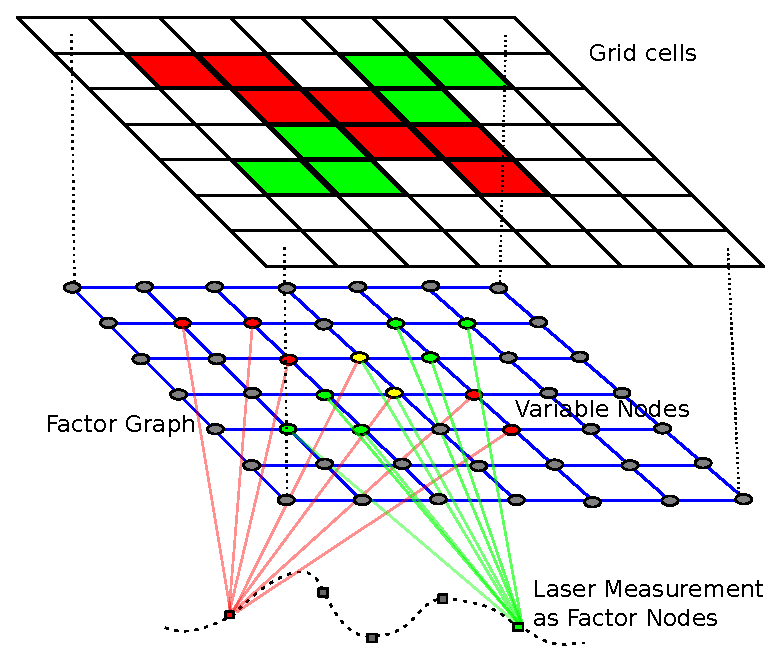
\includegraphics[width=\columnwidth]{../figures/factorgraph/factorgraph.pdf}
  \caption{Representation of occupancy grid mapping as factor graph}
  \label{fig:factor-graph}
\end{figure}

To keep the notation generic and concise we introduce new notation
to rewrite the problems \eqref{eq:fullsolution} and \eqref{eq:mapproblem}
along with factorization obtained in \eqref{eq:modernmap}
\begin{align}
  P_i(x_i = l_i) &= \sum_{\map \in \Omega : x_i = l_i} P(\map) & \forall i \in V
  \label{eq:marginalgeneric}
  \\
     \map* &= \argmax_{\map \in \Omega} P(\map)
  \label{eq:mapgeneric}
  \\
   P(\map) &= \frac{1}{Z}\prod_{f \in F} P_f(\map_f)
  \label{eq:factorizationgeneric}
\end{align}
where  $l_i \in L_i$ denote an element from the label set $L_i$ of node $i \in V$.
Please note the corresponding equivalence of notation, $P_i(x_i = l_i) \equiv p(x_i
= l_i|\measurements, \poses)$, $P(\map) \equiv p(\map|\measurements, \poses)$ and $P_f(\map_f)
\equiv
p(z_f|\map_f, g_f)$.

\section{Markov Chain Monte Carlo Metropolis Hastings}
We implement and evaluate a generalization of Merali's \cite{merali2013icra}
Gibbs sampling algorithm for estimating maps.  Metropolis Hastings is another
popular MCMC algorithm used for sampling from complex probability 
distributions. Gibbs sampling can be shown to be a specialization of Metropolis
Hastings \cite{mackay1998introduction}.

% The class of Markov Chain Monte Carlo (MCMC) methods allow us to sample from
% complex probability distributions. The samples drawn using MCMC
% methods are not independent but correlated as a Markov chain.  They work by
% moving a random walk in the high dimensional space and after sufficient number
% of iterations, it is expected to yield samples from high probability region of the 
% distribution.

Metropolis hastings algorithm requires a \emph{transition probability} $Q(\map'|
\map^r)$, that depends on current sample $\map^r$ and guides
the random walk in the high-dimensional space. We randomly sample a point
$\map'$ from from $Q(.)$ and it is either accepted or rejected based on the
\emph{acceptance probability} $a$:
\begin{align}
  a = \frac{P(\map')Q(\map^r| \map')}
  {P(\map^r)Q(\map'| \map^r)}
\end{align}

If $a \ge 1$, then the new point $\map'$ is accepted otherwise it is accepted with probability $a$. Here acceptance means that the point in next iteration is taken as the sampled point otherwise the older point is retained.
% Mathematically
% \begin{align}
%   \map^{r+1} = \begin{cases}
%     \map' & \text{ if $\map'$ accepted}\\
%     \map^r & \text{ otherwise}\\
%   \end{cases}
% \end{align}
Interested reader is referred to \cite{mackay1998introduction} for further details about the Metropolis Hastings algorithm.

For our experiments, we chose a symmetric uniform transition probability
probability.  We uniformly sample a cell from the map and flip the state of the
sampled cell to get the proposal point $\map'$. This is equivalent to sampling
from the probability density:
\begin{align}
  Q(\map'| \map^r) = \begin{cases}
    \frac{1}{N} & \text{if $\|\map' - \map^r\|_1 = 1$}\\
      0 & \text{ otherwise}
  \end{cases}
  \label{eq:transitionprob}
\end{align}
where $N$ is the number of cells in the map and $\|.\|_1$ is the L1-norm. The
first case in \eqref{eq:transitionprob} enforces that only one cell (or dimension)
in the map can change its state. Since this is a symmetric transition
probability, the acceptance ratio is just the ration of target probabilities.
%We will see this choice is one of the reasons of poor performance of Metropolis Hastings.
Also note that the ratio of probability distributions can be efficiently
computed because of the factorization obtained in
\eqref{eq:factorizationgeneric}:
\begin{align}
  a &= \frac{P(\map')}{P(\map^r)}
    %&= \frac{\prod_{f \in F} P_f(\map'_f)}{\prod_{f \in F} P_f(\map^r_f)}\\
    = \frac{\prod_{f \in n(i)} P_f(\map'_f)}{\prod_{f \in n(i)} P_f(\map^r_f)}
  \label{eq:acceptanceprob}
\end{align}
where $i$ is the (sampled) cell whose state is different in $\map'$ and $\map^r$,
and $n(.)$ denotes the neighborhood of a vertex in graph $G$.  
The above simplification uses the fact that only those terms  that depend on
state of $i$\textsuperscript{th} cell need to be computed. By definition
of graph $G$ only the neighboring factors $f \in n(i)$ depend on state of cell $i$.

It is in general difficult to detect when the sampling algorithm has converged.
In practice, we often run the sampling algorithm for a fixed number of
iterations. Alg.~\ref{alg:metropolis} lists the pseudo code for Metropolis
Hastings algorithm.

% In our experiments, we use this sampling method as a representative of Merali et al
% \cite{merali2013icra} work.
% Also note that Gibbs sampling is a special case of Metropolis Hastings and our
% implementation of Metropolis Hastings for a binary variable exactly matches the
% Gibbs sampling because acceptance ratio evaluates to the conditional
% probability $\frac{P(x'_i|\map_{\neg i})}{\map_P(x^r_i|\map_{\neg i})}$ that 

% Now, we know that $\map'$ and $\map^r$ differ only by one cell or dimension, say $i$. Using this fact we can assert that only those subsets $\map_f$ of map can be different that contain
% 
\begin{algorithm}
  \KwData{
  Factor Graph $G = (V, F, E)$\;
  %Label set $\{\Sx\}_{i \in V}$\;
  %Step size $\alpha > 0$\;
  Maximum number of iterations $N$\;
  }
  \KwResult{$\map^r$}
  Initialize the map $\map^0$ randomly.\;
  $r = 0$\;
  \While {$r < N$} {
    Randomly choose a cell $i : i \in V$\;
    Flip its state $x'_i = \neg x^r_i$ in $\map^r$ to get $\map'$\;
    Compute acceptance probability $a$ by \eqref{eq:acceptanceprob}\;
    Sample random number $q : 0 \le q \le 1$\;
    \If {$a \ge 1$ or $a \ge q$} {
      Accept proposed point, $\map^{r + 1} = \map'$\;
    } \Else {
      Reject proposed point, $\map^{r + 1} = \map^r$\;
    }
    $r \leftarrow r + 1$\;
  }
  \caption{Metropolis Hastings}
  \label{alg:metropolis}
\end{algorithm}

\subsection{Heat map}
As we uniformly sampled cells from the map, we noticed that not all
cells are equally important in mapping. There are three kinds of region any
occupancy map, occupied, free and unexplored. Sampling and analyzing a cell in
unexplored region is not much helpful as we do not have any evidence for the
region. On the other hand, the central regions of free areas are not very
interesting as all factors usually agree on their state. The uncertainty lies
usually lies along the boundaries of free and occupied regions. This is the
region we want to focus on.

We employ a \emph{heat map} to bias our sampling along the boundaries of free
and occupied regions. We maintain a vector of cells $\map_h$ that form the
``interesting'' region of the map. In our experiments, we take the last cell
spanned by each laser measurement as an ``interesting'' cell and add it to the
\emph{heat map}, $\map_h$. We use a sampling bias of $1:4$ for cells
outside heat map to cells within heat map. We compare both Metropolis Hastings
with and without heat map in our experiments.

\section{Modern inference algorithms}
As discussed in Sec.~\ref{sec:related}, last decade saw a spurt in faster and
more accurate MAP inference algorithms \cite{kappes2013comparative}. Because of
their ability to handle higher order factors
\cite{potetz2007efficient,komodakis2009beyond}, we evaluate belief propagation
and dual decomposition on the problem of occupancy grid mapping.

\subsection{Belief Propagation}
\newcommand{\bpmsg}[4]{\mu^{#4}_{#1\rightarrow#2}(#3)}
% TODO: Use introduction section of \cite{potetz2007efficient} to introduct belief propagation specifically 
Sum product algorithm over factor graphs \cite{kschischang2001factor} is a
powerful yet simple algorithm to compute marginals  of
expression (of the form \eqref{eq:fullsolution}) that can be decomposed into
factors of the form \eqref{eq:modernmap}. The algorithm provides exact
marginals in the case when the graphs have no loops. For general case the
algorithm has been shown %TODO: cite?  
to converge in most of the practical problems.
 
%The sum product algorithm is one of the easiest algorithm to implement. 
The sum product algorithm works by sending messages along the edges of factor
graph. The messages can be understood as a belief of the source node
considering all other neighbors except the destination. These messages are
defined on a directed edge, with a different message value for each state of
the variable node involved. 

Let $\bpmsg{f}{i}{l_i}{r}$ represent message from
node $i \in V$ to node $f \in F$ for state $x_i = l_i$ at any iteration $r$ of the
algorithm. With a similar convention we take $\bpmsg{i}{f}{l_i}{r}$ to denote
update in opposite direction. We use the following equations to update the messages depending whether the direction of edge is from variable node to factor node or vice versa:
\begin{align}
  \bpmsg{f}{i}{l_i}{r+1} &= \sum_{\map_f \in \Omega_f: x_i = l_i}P_f(\map_f)\prod_{j \in n(f) \setminus i}\bpmsg{j}{f}{x_j}{r}
  \label{eq:factor2node}
  \\
  \bpmsg{i}{f}{l_i}{r+1} &= \prod_{h \in n(i) \setminus f}\bpmsg{h}{i}{l_i}{r}
  \label{eq:node2factor}
\end{align}
where $\Omega_f = \prod_{i \in n(f)} L_i$ denotes the sample space of the
neighborhood of factor $f$ in graph $G$. On convergence the belief of variable
nodes can be computed by the product of incoming messages:
\begin{align}
  P(x_i = l_i) &= \prod_{f \in n(i)}\bpmsg{f}{i}{l_i}{r}
\end{align}
This is called the \emph{sum-product} belief propagation (BP) algorithm.

One can compute the maximizing assignment instead of marginals by computing
the max-product instead of sum product in \eqref{eq:factor2node} and finally 
choosing the maximizing assignment of incoming messages:
\begin{align}
  \bpmsg{f}{i}{l_i}{r+1} &= \max_{\map_f \in \Omega_f: x_i =
l_i}P_f(\map_f)\prod_{j \in n(f) \setminus i}\bpmsg{j}{f}{x_j}{r}\\
x_i^* &= \argmax_{x_i \in L_i} \prod_{f \in n(i)}\bpmsg{f}{i}{l_i}{r}.
\end{align}
This form of the algorithm is called \emph{max-product} BP.

Belief propagation was initially designed to work on factor graphs without
loops. In such a case one can start message update from the leaf nodes and
a node can be ``triggerred'' to pass on the messages when messages from all 
but one neighbors are available. However, for graphs with loops various update
sequences have been suggested that vary from problem to problem. For example,
in vision problems, where the factor graph is a 2D grid, horizontal and then
vertical sweeps has been shown to produce good results.
For our implementation, we choose random update sequence i.e. a random edge is
selected from the graph for each iteration of message update.

\subsection{Subgradient Dual decomposition}
\newcommand{\msg}[3]{\mu_{#1#2}(#3)}
\newcommand{\assign}{\leftarrow}
\newcommand{\Sx}{L_i}

Dual decomposition algorithm employs Lagrangian relaxation technique from
integer programming to minimize. Here we explain the implementation of the
algorithm without going into mathematical proofs. Interested user is
referred to
\cite{sontag2011introduction,jojic2010accelerated,komodakis2009beyond} for
proofs and more variations of the algorithm. 

The underlying idea for dual decomposition is to split the maximization
problem into \emph{slave} problems that can be efficiently maximized. In a
factor graph formulation the natural \emph{slave} problem is one corresponding
to each factor:
\begin{align}
  \map^f &= \argmax\limits_{\map^f} P_f(\map^f)
  \prod\limits_{i \in n(f)}\exp\left(-\msg{i}{f}{x^f_i} \right)
\end{align}
where $\map^f = \{x_i^f\}_{i \in n(f)}$ is the optimum assignment 
as determined by the corresponding \emph{slave}
problem. And $\msg{i}{f}{x^f_i}$ is the message (also the Lagrangian
multiplier) from node $i$ to $f$ about state $x^f_i$. 
The above slave problem is usually written in the form of 
negative log likelihood:
\begin{align}
  \map^f &= \argmin\limits_{\map^f} \theta_f(\map^f)
  +\sum\limits_{i \in n(f)}\msg{i}{f}{x^f_i}
  \label{eq:slavemin}
\end{align}
where $\theta_f(\map^f) = -\log P_f(\map^f)$ is the negative log
likelihood corresponding to the factor.

In each iteration of the algorithm all slave problems are allowed to choose
their optimum assignment independently. If all the factors agree on the
assignments, then we have reached the global optima. Often this is
not the case. In case of disagreement, we decrease the belief of all the
disagreeing slave problem in about their respective optimums by sending
appropriate messages. It can be shown that as long as we can increase the
messages by decreasing step size in each iteration, the algorithm is guaranteed
to converge to an approximate solution of the original problem
\cite{sontag2011introduction}.

Pseudo code for dual decomposition (DD) is provided in
Alg~\ref{alg:dualdecompostion}. Apart from input factor graph $G = (V, F, E)$
and label set $\{\Sx\}_{i \in V}$ introduced in Sec~\ref{sec:notation}, dual
decomposition depends on a step size $\alpha$.

\begin{algorithm}
  \DontPrintSemicolon
  \KwData{\;
  Factor Graph $G = (V, F, E)$\;
  %Label set $\{\Sx\}_{i \in V}$\;
  Step size $\alpha > 0$\;
  Maximum number of iterations $N$\;
  }
  \KwResult{Labels $\{x^f_i\}_{(i, f) \in E} $,
  Messages $\{\msg{i}{f}{x_i}\}$}

  $\msg{i}{f}{x_i} \assign 0 \hfill \forall (i, f) \in E, x_i \in \Sx$\;
  $r \assign 1$\;
  \While{$r < N$} {
    %\tcp{For disagreeing factors}
    \For {$f \in F$} {% : \exists i, i' \in n(f) : x_i^f \ne x_{i'}^f$} {
      $\map^f \assign \argmin\limits_{\map^f} \left( \theta_f(\map^f) + \sum\limits_{i \in n(f)}\msg{i}{f}{x^f_i} \right)$\;
      %$\map^f \assign \argmax\limits_{\map^f} P_f(\map^f)
      %\prod\limits_{i \in n(f)}\exp\left(-\msg{i}{f}{x^f_i} \right)$\;
    }
    \tcp{For disagreeing nodes}
    \For {$i \in V : \exists f, f' \in n(i) : x_i^{f'} \ne x_i^f$} {
      \For{$f \in n(i)$}{
        $\msg{i}{f}{x^f_i} \assign \msg{i}{f}{x^f_i} + \frac{\alpha}{r}$\;
      }
    }
    $r \leftarrow r + 1$\;
  }
  \label{alg:dualdecompostion}
  \caption{Subgradient Dual Decomposition}
\end{algorithm}
Upon convergence or completing maximum number of iterations, we can compute the
optimal assignment for variable nodes with disagreeing \emph{slave} from the
messages:
\begin{align}
  x_i &= \argmax\limits_{x_i \in \Sx} \sum\limits_{f \in n(i)}\msg{i}{f}{x_i}.
\end{align}
Note that the above equation is only valid for disagreeing \emph{slaves}. When the 
the \emph{slaves} agree, we can simply pick the agreed upon value.

Note that the Subgradient DD algorithm depends on a parameter step size. We
note that step size is important attribute and affects the speed of the
algorithm. To illustrate that we show the convergence of dual decomposition
with different step size on \emph{cave} dataset in
Fig.~\ref{fig:dualdecomposition-stepsize}. Note that erring on higher side
causes oscillations, while erring lower side can cause convergence to be too
slow.

Another limitation of dual decomposition is an optimization algorithm, hence it
only solves the MAP problem \eqref{eq:mapgeneric}, but not the marginal problem
\eqref{eq:marginalgeneric}.

%\subsection{Selection of step size}
% \section{Belief propagation with disagreement tracking}
% Intuitively, dual decomposition converges faster because it focuses on the disagreeing 

\section{Higher order factors and efficiency}

The message update equation \eqref{eq:factor2node} in BP algorithm is
exponential in the size of neighborhood of factor $f$. Observing that the
neighbourhood size in our factor graph formulation can go up to hundreds to
thousands of nodes; computing all such terms will be computationally
expensive. Same is true for slave minimization \eqref{eq:slavemin} in DD algorithm.
% If the range observation is 30m in an
% occupancy grid with cell size of 10cm, the neighborhood size would be
% approximately 300 and the sample space of neighboring nodes $\Omega_f$ will be
% of the order $2^{300}$.

In this section, we seek a generic class of factors that can be 
efficiently applied to the belief propagation (BP) and dual decomposition (DD)
algorithms. We begin by introducing common forward sensor models, that need to
fit our class of factors followed by their generalization and then their 
application to the BP and DD algorithms.

\begin{comment} % May be move to experiments section
Sensor models are mathematical representations of relationship between environment and sensor reading. We discuss here the sensor models that we use for our experiments.

\subsection{Inverse sensor model}
Inverse sensor model describes the environment given the sensor reading. We use
the following inverse sensor model \cite{merali2013icra}
\begin{align}
  p(x_i=1|z_f, g_f) &= \begin{cases}
  p_{\text{free}} & \text{ if $i \in n(f)_{1:-1}$}\\
  p_{\text{occupied}} & \text{ if $i = n(f)_{-1}$}\\
                  0.5 & \text{ otherwise}
  \end{cases},
\end{align}
where $n(f)_{1:-1}$ denotes all but last cell traversed by the laser,
$n(f)_{-1}$ denotes the last cell reached by laser, $p_{\text{free}} = 0.0588$
and $p_{\text{occupied}} = 0.9411$ are probabilities associated with the cell
being free and occupied respectively. The constant probability values used
here are computed from log odds values provided by Merali et al.
\cite{merali2013icra}.

\end{comment}

\subsection{Forward sensor models}
\label{sec:forward}
Forward sensor models estimate the sensor reading given the environment.
Hence, these models can be more close the actual behaviour of the sensors.
In this section we describe consider two commonly used sensor models.

\subsubsection{Gaussian sensor model}
\newcommand{\actz}{\bar{z}_f(\map_f, g_f)}
In this sensor model, we assume that the laser measurements are affected by
Gaussian noise. The forward sensor model is given by
\begin{align}
  p(z_f|\map_f, g_f) &=
  \frac{1}{\sqrt{2\pi}\sigma}\exp\left(-\frac{(\actz - z_f)^2}{2\sigma^2}\right)
  \label{eq:gaussiansensormodel}
\end{align}
where $\actz$ is the distance of first occupied cell in $\map_f$ starting
from pose $g_f$. Also $\sigma$ is a measure of noise in laser measurement and
it often depends on the distance measured. For our experiments we assume noise
to linearly vary with distance as $\sigma = \sigma_0z_f$. 

% In terms of negative log likelihood, the energy function becomes
% \begin{align}
%   \theta_f(\map_f) &= \frac{1}{2\sigma_0^2}\left(1 -
%   \frac{\actz}{z_f}\right)^2 + \log(\sqrt{2\pi}\sigma_0z_f)
% \end{align}

\subsubsection{Piecewise constant sensor model}
It is common in graphical models to have very simple factors that assign high
probability to expected configuration and very low probability to all other
states. 
% A sensor model on these lines would look like
% \begin{align}
%   p(z_f|\map_f, g_f) &= \frac{1}{Z}\begin{cases}
%               1 & \text{ if } \map_f = [0, 0 \dots 0, 1]^\top\\
%     \exp(-1000) & \text{ otherwise}
% \end{cases}
% \end{align}
%where $Z$ is the normalization constant and $[0, 0 \dots 0, 1]$ means that all
%cells are $0$ except the last cell which is $1$. 
%In this context, we consider
%$\map^f$ to be a vector of ordered cell labels through which laser
%measurement $f$ passes.
%
However, we chose to prefer free space over occupied ones. Hence, we come with
the following energy function that we use in all our experiments.
\begin{align}
  p(z_f|\map_f, g_f) &= \frac{1}{Z}\begin{cases}
                       1 & \text{ if } \map_f = \vect{R}_{f1}\\
              \exp(-900) & \text{ if } \map_f = \vect{R}_{f2}\\
           \exp(-1000) & \text{ otherwise}
  \end{cases}
  \label{eq:piecewiseconstant}
\end{align}
where $Z$ is the normalization constant $\vect{R}_{f1} = [0, 0 \dots 0,
1]^\top$ denotes all free but last occupied cell pattern and $\vect{R}_{f2} =
[0, 0 \dots 0, 0]^\top$ denotes all free cells.

\subsection{Generalization to Pattern-based factors}
\label{sec:patternfunctions}

% We can efficiently compute \eqref{eq:factor2node} for certain class of
% $P_f(.)$. 
We define a consider a class of \emph{pattern-based} higher order factors that
are a generalization of those discussed by Komodakis et al.
\cite{komodakis2009beyond}. These are factors of the form:
\begin{align}
  P'_f(\map_f) = \begin{cases}
    \psi_{m} & \text{ if $\map_f \sim \vect{R}_m$} \,\,\, \forall 1 \le m \le M\\
    \psi_{\text{min}} & \text{ otherwise}
  \end{cases}
  \label{eq:patternfunction}
\end{align}
where $\vect{R}_m$ is one of the mutually exclusive $M$ patterns and
expression $\map_f \sim \vect{R}_m$ denotes that vector $\map_f$
``matches'' pattern $\vect{R}_m$.  
%Usually $M$ is either a constant or linear in the size of neighborhood $n(f)$.
%We further constrain the class of functions by requring each pattern
A pattern, $\vect{R}_m = (n^m_0(f), \vect{r}^m)$, is defined by a non empty set
of \emph{fixed} nodes $n^m_0(f) \subseteq n(f)$ that are supposed to have
desired values $\vect{r}^m$, while the state of remaining \emph{free} nodes
$n^m_*(f) = n(f) \setminus n^m_0(f)$ can have any values from the label set 
and they do not affect factor value $P_f(\map_f)$. A configuration
$\map_f$ ``matches`` pattern $\vect{R}_m$ if the state of \emph{fixed}
nodes in same as desired values, $x_i = r_{mi} \forall i \in n^m_0(f)$.
For efficient computation we assume that number of patterns $M$ is much
smaller than the sample space $\Omega_f$.

It is clear that piecewise constant sensor model \eqref{eq:piecewiseconstant}
is an instance of pattern based functions. It is also possible to represent
Gaussian sensor model \eqref{eq:gaussiansensormodel} as a pattern based
factor. We use the fact that
the term $\bar{z}_f(\map_f, g_f)$, just depends on first occupied cell. We
define pattern $\vect{R}_m$ such that the first occupied cell is
$m$\textsuperscript{th} cell in $n(f)$:
\begin{align}
  n^m_0(f) &= n(f)_{1:m}\\
\vect{r}^m &= \{ r^m_{i} = 0 \}_{i \in n(f)_{1:m-1}} \text{ and } r^m_{n(f)_m} = 0\\
       R_m &= (n^m_0, \vect{r}^m)
\end{align}
where $n(f)_{k}$ is the $k$\textsuperscript{th} cell that is traced by laser. With
this formulation, we will have $M = n(f)$ patterns to describe the gaussian
sensor model in the form \eqref{eq:patternfunction} with $\psi_m$ given by
\begin{align}
  \psi_m &= \frac{1}{\sqrt{2\pi}\sigma}\exp\left(-\frac{(\delta(m)- z_f)^2}{2\sigma^2}\right)
\end{align}
where $\delta(m)$ is the distance of $m$\textsuperscript{th} cell from robot
starting point $g_f$. Also note that in this formulation the only case for
\emph{otherwise} is the one when all cells are $0$ (or free).

%The first two cases of
%\eqref{eq:piecewiseconstant} are already in pattern-based format, but the
%otherwise case is not mutually exclusive with 

\subsection{Efficient sum product}
% We note that for Occupancy grid mapping the neighborhood of nodes in factor
% graph $G$ can be large. For example a typical laser scan might have maximum
% range of up to 50 m, which can cover up to 500 cells event at 10cm resolution.
% In such a factor graph, even the sample space $\Omega_f$ of neighbors
% $n(f)$ of factor $f$ can be very large; of the order of $2^{500}$  in above
% example. This makes message update step in \eqref{eq:factor2node}
% computationally expensive.

To efficiently compute \eqref{eq:factor2node} for pattern-based factors
defined %Section~\ref{sec:patternfunctions},
we need the messages to be
normalized. The messages $\bpmsg{i}{f}{l_i}{r}$ are can be easily normalized
over the label set $L_i$ to sum up to one:
\begin{align}
  \sum_{l_i \in L_i} \bpmsg{i}{f}{l_i}{r} = 1
\end{align}

Now, the messages are a valid probability measure for source variable node.
Using this property, we can efficiently compute \eqref{eq:factor2node}. We
compute the probability of each pattern being true
%as beliefs $\bpmsg{i}{f}{x_i}{r}$
% \begin{align}
%   p(\vect{x_f} \sim \vect{R}_m) 
%   %= \sum_{\vect{x_f} \sim \vect{R}_m} \prod_{j \in n(f)}\bpmsg{j}{f}{x_j}{r}\\
%   %&= \prod_{j \in n^m_0(f)}\bpmsg{j}{f}{R_{mj}}{r}\underbrace{\sum_{\map^*_f \in \Omega^*_f}\prod_{j \in n^m_*(f)}\bpmsg{j}{f}{x_j}{r}}_{=1\text{, because $\vect{R}_m$ do not contraints $n^m_*(f)$}}\\
%   %&= \prod_{j \in n^m_0(f)}\bpmsg{j}{f}{R_{mj}}{r}\left(\sum_{\vect{x_f} \sim \vect{R}_m}\prod_{j \in n^m_*(f)}\bpmsg{j}{f}{x_j}{r}\right)
%   &= \prod_{j \in n^m_0(f)}\bpmsg{j}{f}{R_{mj}}{r}
% \end{align}
% where $R_{mj}$ is the fixed value of $j$\textsuperscript{th} node in pattern 
% $\vect{R}_m$.
%The summation inside the bracket evaluates to one, because
%$\map_f \sim \vect{R}_m$ do not constraints state of any node in $n^m_*(f)$
%by definition. 
The probability of pattern is just the product of beliefs of \emph{fixed}
terms as \emph{free} nodes can take any value
\begin{multline}
  p(\vect{x_f} \sim \vect{R}_m|x_i = l_i) \\
  = \begin{cases}
0 & \text{if $i \in n^m_0(f)$ and $l_i \ne r^m_i$}\\
  \prod\limits_{j \in n^m_0(f) \setminus i}\bpmsg{j}{f}{r^m_j}{r} & \text{otherwise}
  \end{cases}
\end{multline}

% Note that we have not treated the node being marginalized specially.  Unlike
% \eqref{eq:factor2node}, we do not leave out target node $i$ from product
% terms, instead we temporarily replace the beliefs $\bpmsg{i}{f}{x_i}{r}$ with
% deterministic values to achieve the same effect
% \begin{align}
%   \bpmsg{i}{f}{x_i}{r} = \begin{cases}
%     1 & \text{if $x_i = l_i$}\\
%     0 & \text{otherwise}
%   \end{cases}
% \end{align}
%Note that probabiltiy $p(\vect{x_f} \sim \vect{R}_m)$, depends only on the fixed nodes $n^m_0(f)$.
Now, we are in position to efficiently compute \eqref{eq:factor2node}
\begin{multline}
  \bpmsg{f}{i}{l_i}{r+1} = \sum_{m \le M} \psi_m p(\vect{x_f} \sim \vect{R}_m|x_i = l_i)
  + \psi_{\text{min}} p_{\text{otherwise}}
  \label{eq:efficientbp}
\end{multline}
where $p_{\text{otherwise}} = 1 - \sum_{m \le M}p(\vect{x_f} \sim \vect{R}_m|x_i = l_i)$.

The message update can be computed in $O(M|n(f)|)$ using \eqref{eq:efficientbp}, instead of $O(L_i^{n(f)-1})$ in the general case.

\subsection{Efficient dual decomposition}
In similar lines of BP, slave minimization \eqref{eq:slavemin} in dual
decomposition can be done efficiently for \emph{pattern-based} factors.
We note that slave function is composed of two terms, the factor itself and
the messages. Since the factor is a pattern based function, we can address
the minimization for each pattern and later taking the minima of minimums for
all patterns. While minimizing for a pattern we can make use of the fact that
the value of $\theta_f$ is constant for a pattern and hence we need to focus
only on minimizing the messages. Minimizing messages is trivial by
as each term can be minimized independently.

Minimizing the \emph{otherwise} case of patterns can be tricky as naive
minimization can result in values that matches one of the explicit patterns.
Depending on how big we expect the space of \emph{otherwise} case to be, we
can approach it in two different ways.  If the space for \emph{otherwise} case
is small (like in the gaussian sensor model), we simply go over all the entire
sample space to find minimum value. Otherwise, we depend on the sample space
covered by patterns being small. In this case we keep finding n-best
minimizations of messages until we get a minimization that does not match any
of the patterns already considered.  
For example, in case of piecewise constant sensor model, there are only two
patterns that need to be checked for exclusion. The otherwise term can be
easily minimized by finding three best assignments that minimize the messages
term.

\section{Experiments} 
We run experiments on simulated as well real data.
The simulated data is generated using \emph{Player/Stage} \cite{gerkey2003player}
project. We use multiple map bitmaps bundled along with player/stage library.
The robot motion is generated using the wander driver. The robot is allowed to
wander in the map for 2 minutes aggregating approximately 270,000 laser measurements.
The qualitative results are shown in
Fig.~\ref{fig:convergence-comparison-visuals} for several simulated dataset. To
evaluate the convergence rate of each algorithm, we plot total energy of the
graph with respect CPU ticks taken by the algorithm. The plot of energy
convergence with respect to time for cave dataset is shown in
Fig.~\ref{fig:convergence-comparison}.

For real data, we have used the \emph{albert-b-laser} dataset provided by
Cyrill Stachniss from University of Freiburg. The dataset was captured by a
B21r robot with a SICK PLS moving through a lab at University of Freiburg.
This data set was obtained from the Robotics Data Set Repository
(Radish)~\cite{howard2003radish}. Thanks go to Cyrill Stachniss for providing
this data.

In all our experiments we do not use any occupancy prior. Although, Merali et
al \cite{merali2013icra} suggest using an occupancy prior of 0.3 for better
convergence. We use a step size of 50 for dual decomposition and piecewise constant 
sensor model.

\section{Conclusion}
We note that sampling algorithms are liable to getting stuck in a local minima
because we flip only one cell at a time. Even from the qualitative results for
sampling based algorithm, we see that the walls are thinner than corresponding
results in other algorithms which shows the inability of sampling based
algorithms to form lower energy thicker walls for piecewise constant sensor
model.

We note that dual decomposition is faster because it focuses on disagreeing
nodes. However, step size is crucial parameter that affects speed of
convergence. On the other hand sum product belief propagation do not depends
on any parameter factor, but has no preference for the disagreeing nodes.
This combination obviously hints towards an algorithm where we perform 
belief propagation over disagreeing nodes only. The state of art variations 
of these algorithms like Sequential Tree Re-Weighted (TRW-S) belief
propagation \cite{kolmogorov2006convergent}, accelerated dual Decomposition
\cite{jojic2010accelerated} are step in this direction.
However, even without using the state of art optimum algorithms since we get
better performance than sampling methods. This only serves to prove our
assertion that modern inference methods should be used occupancy grid mapping 
when computation time is not a limiting factor.


\showcaptionsetup{subfloat}
\begin{figure*}
  % TODO: Fix graph to converge at the same time
  \subfloat[Convergence on cave dataset]{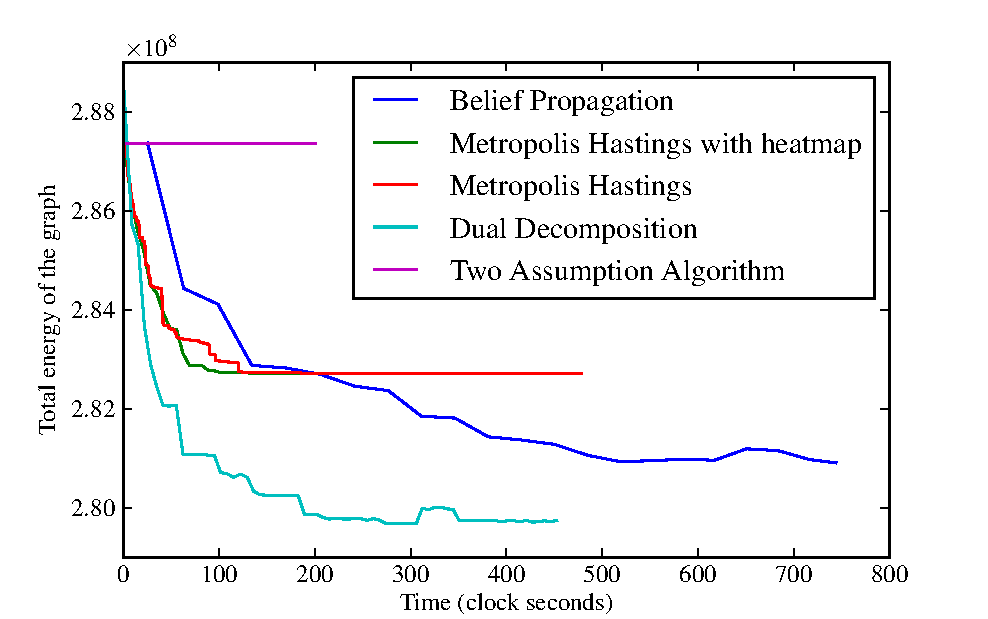
\includegraphics[width=0.30\textwidth]{../figures/relativeconvergence.pdf}}%
  \subfloat[Convergence on hospital section dataset]{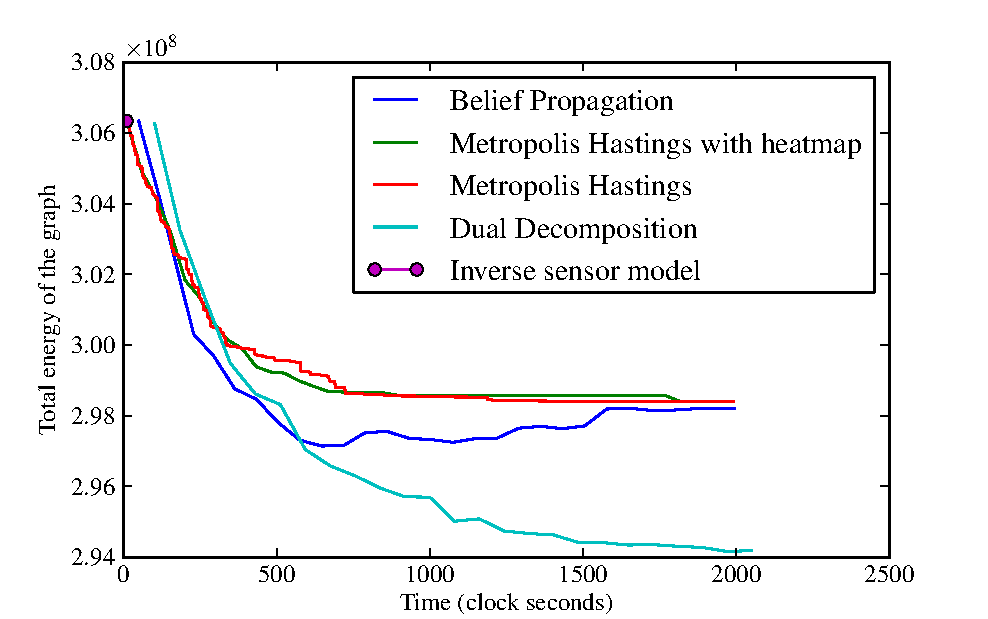
\includegraphics[width=0.30\textwidth]{../../Data/hospital_section_player/plot-time-energy.pdf}}\\
  \subfloat[Convergence on hospital dataset]{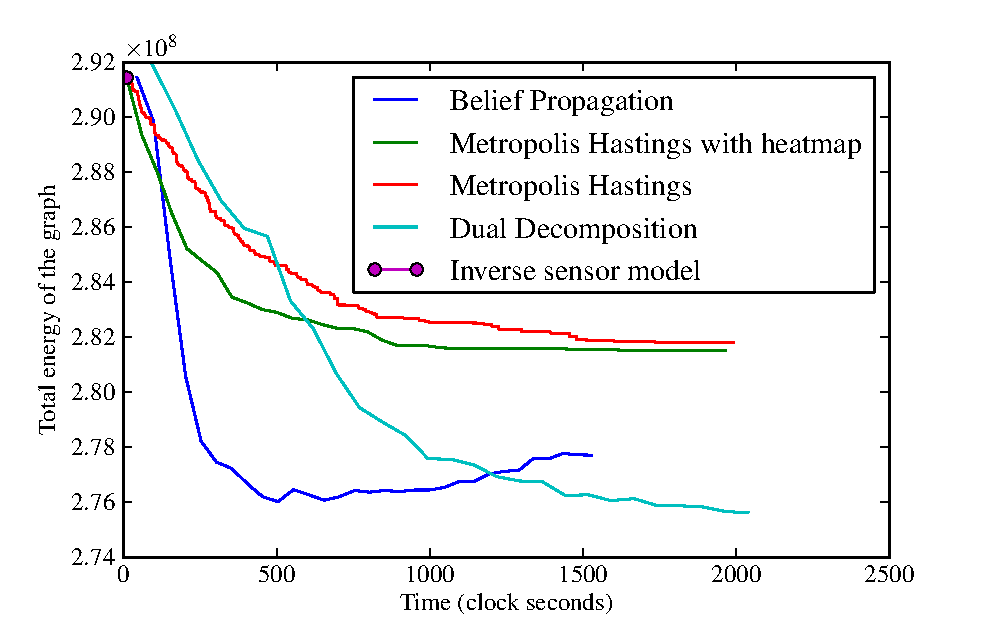
\includegraphics[width=0.30\textwidth]{../../Data/hospital_player/plot-time-energy.pdf}}%
  \subfloat[Convergence on albert-b dataset]{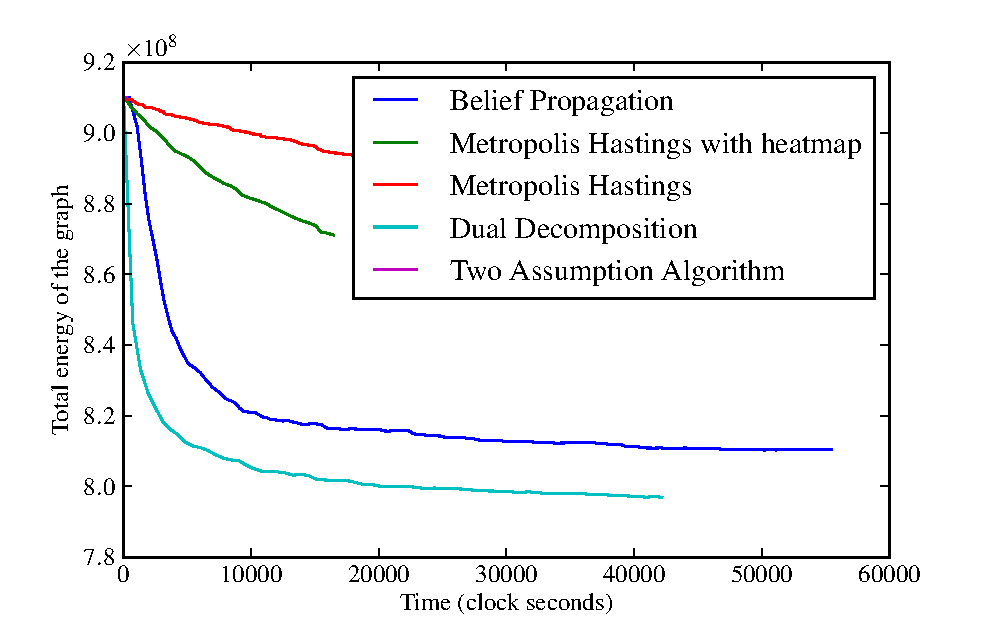
\includegraphics[width=0.30\textwidth]{../figures/convergence-albert-b.pdf}}%
  \subfloat[Convergence with different step size in dual decomposition]{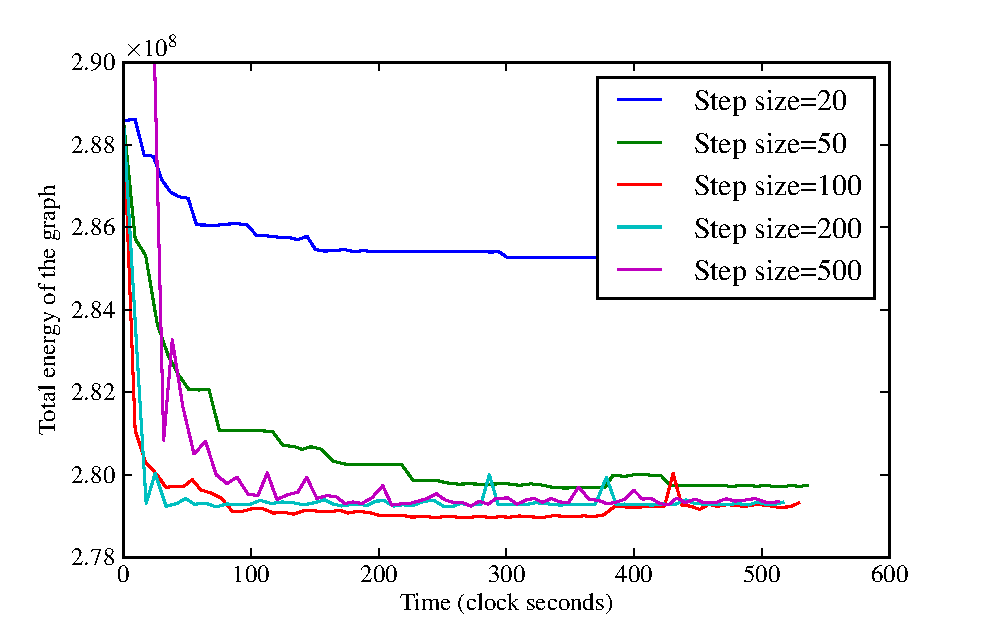
\includegraphics[width=0.30\textwidth]{../figures/dualdecomposition-stepsize-inc500.pdf}}
  \caption{Comparison of convergence of different algorithms on occupancy grid graph. While sampling methods like Metropolis hastings converge quickly they stay far from optimum energy. On the other hand modern minimization algorithms reach closer to an optimum value.}
  \label{fig:convergence-comparison}
\end{figure*}
  %\caption{The rate of convergence in dual decomposition depends on step size}
  %\label{fig:dualdecomposition-stepsize}
\begin{figure*}
  %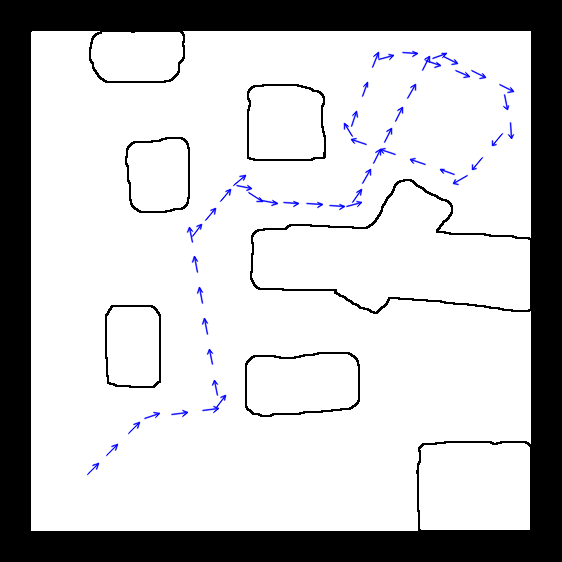
\includegraphics[width=0.2\textwidth]{../figures/cave_trajectory.png}%
  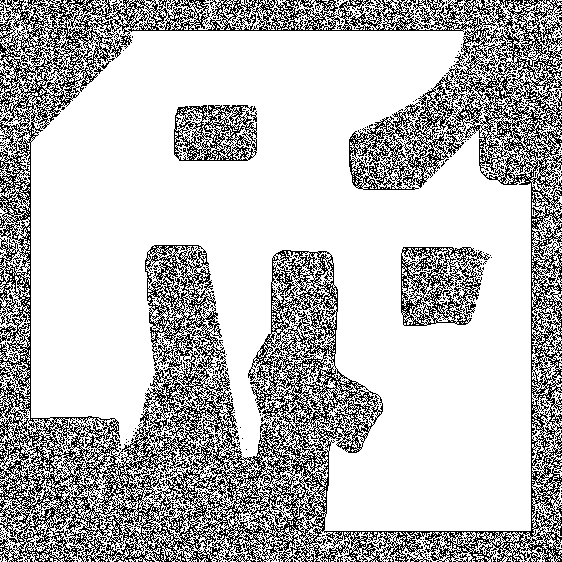
\includegraphics[width=0.16\textwidth]{../../Data/cave_player/gt-final.png}%
  
\includegraphics[width=0.16\textwidth]{../../Data/cave_player/TwoAssumptionAlgo.png}%
  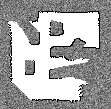
\includegraphics[width=0.16\textwidth]{../../Data/cave_player/SICKSlowMetropolis.png}%
  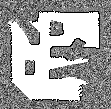
\includegraphics[width=0.16\textwidth]{../../Data/cave_player/SICKDDMCMC.png}%
  
\includegraphics[width=0.16\textwidth]{../../Data/cave_player/run_belief_propagation.png}%
  
\includegraphics[width=0.16\textwidth]{../../Data/cave_player/dualdecomposition.png}\\
  
\includegraphics[width=0.16\textwidth]{../../Data/hospital_player/gt-final.png}%
  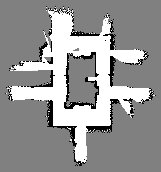
\includegraphics[width=0.16\textwidth]{../../Data/hospital_player/TwoAssumptionAlgo.png}%
  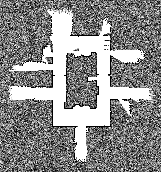
\includegraphics[width=0.16\textwidth]{../../Data/hospital_player/SICKSlowMetropolis.png}%
  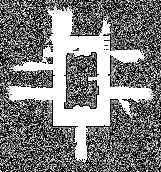
\includegraphics[width=0.16\textwidth]{../../Data/hospital_player/SICKDDMCMC.png}%
  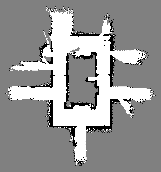
\includegraphics[width=0.16\textwidth]{../../Data/hospital_player/run_belief_propagation.png}%
  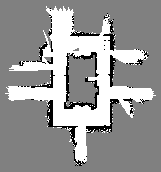
\includegraphics[width=0.16\textwidth]{../../Data/hospital_player/dualdecomposition.png}\\
  %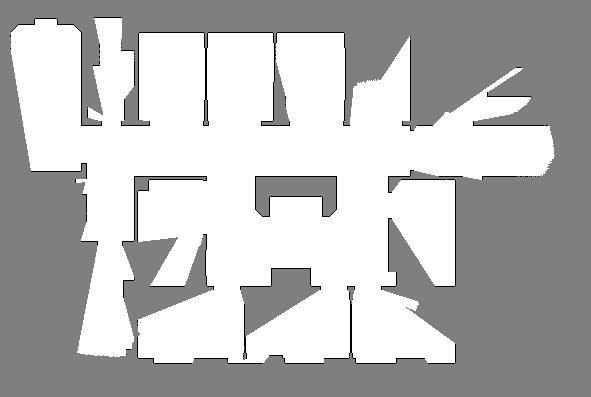
\includegraphics[width=0.16\textwidth]{../../Data/hospital_section_player/gt-final.png}%
  % 
\includegraphics[width=0.16\textwidth, trim=0 0 0 3px, clip]{../../Data/hospital_section_player/TwoAssumptionAlgo.png}%
  % 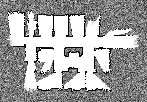
\includegraphics[width=0.16\textwidth, trim=0 0 0 3px, clip]{../../Data/hospital_section_player/SICKSlowMetropolis.png}%
  % 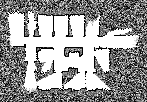
\includegraphics[width=0.16\textwidth, trim=0 0 0 3px, clip]{../../Data/hospital_section_player/SICKDDMCMC.png}%
  % 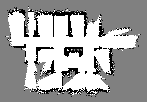
\includegraphics[width=0.16\textwidth, trim=0 0 0 3px, clip]{../../Data/hospital_section_player/run_belief_propagation.png}%
  % 
\includegraphics[width=0.16\textwidth, trim=0 0 0 3px, clip]{../../Data/hospital_section_player/dualdecomposition.png}\\
  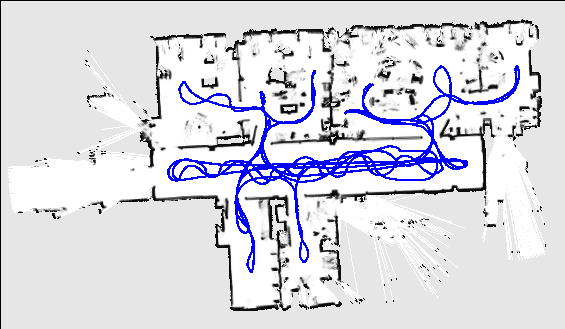
\includegraphics[height=0.16\textwidth,                                   angle=90]{../../Data/albertb.sm/path.png}%
  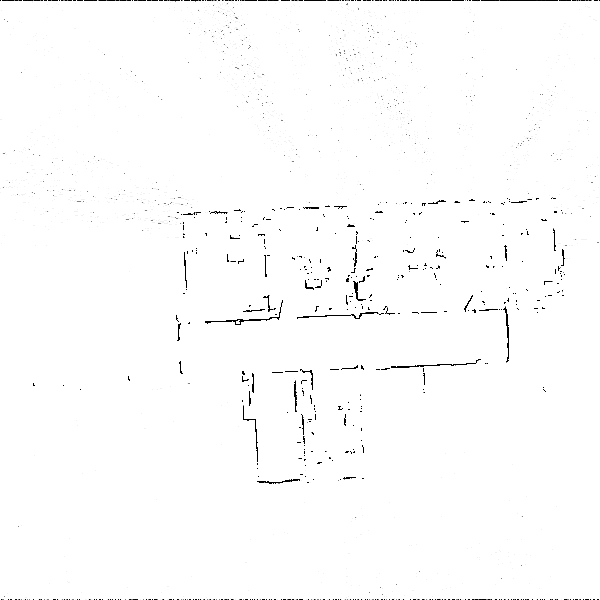
\includegraphics[height=0.16\textwidth, trim=65px 125px 20px 175px, clip, angle=90]{../../Data/albertb.sm/TwoAssumptionAlgo.png}%
  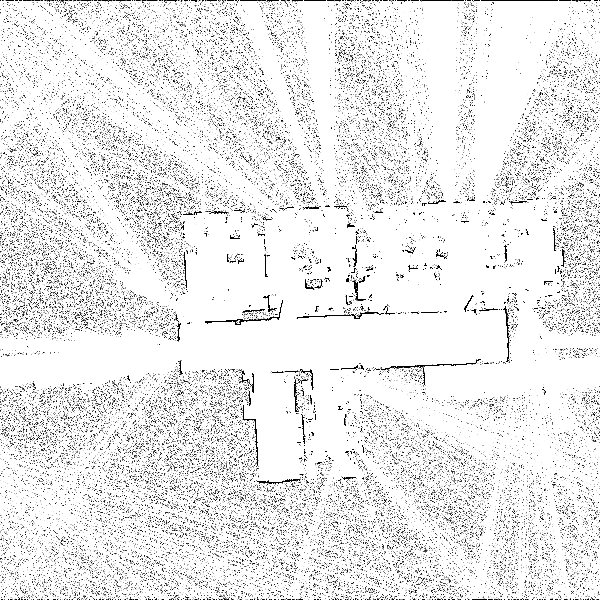
\includegraphics[height=0.16\textwidth, trim=65px 125px 20px 175px, clip, angle=90]{../../Data/albertb.sm/SICKSlowMetropolis.png}%
  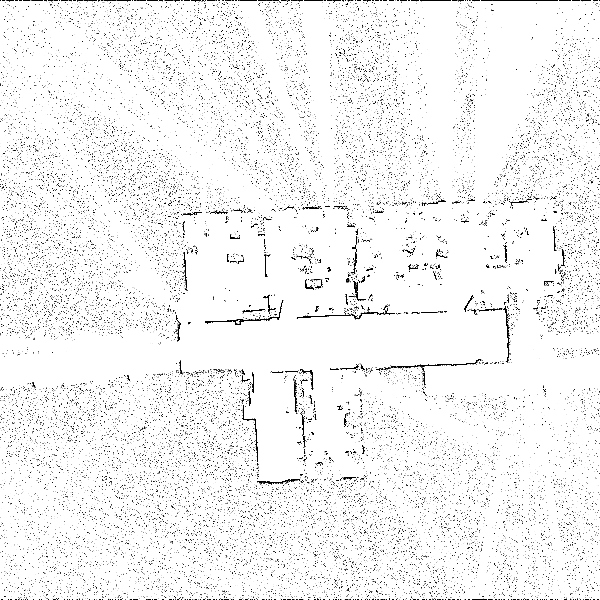
\includegraphics[height=0.16\textwidth, trim=65px 125px 20px 175px, clip, angle=90]{../../Data/albertb.sm/SICKDDMCMC.png}%
  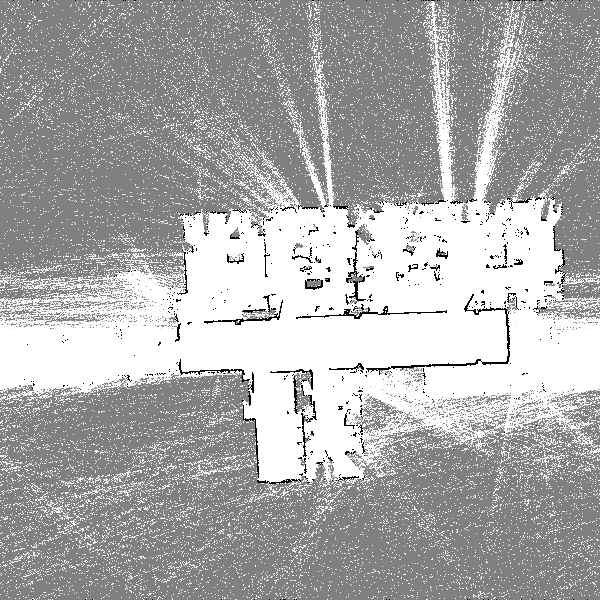
\includegraphics[height=0.16\textwidth, trim=65px 125px 20px 175px, clip, angle=90]{../../Data/albertb.sm/run_belief_propagation.png}%
  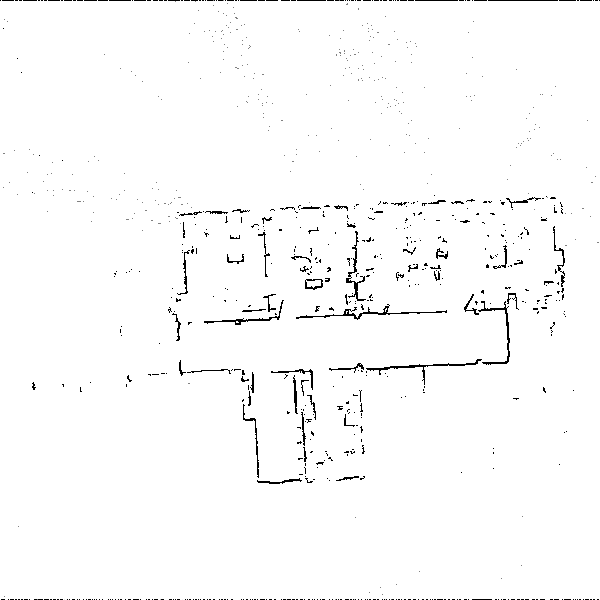
\includegraphics[height=0.16\textwidth, trim=65px 125px 20px 175px, clip, angle=90]{../../Data/albertb.sm/dualdecomposition.png}%
  \caption{Qualitative results (from left to right) a) Ground truth with the trajectory of the robot b) Two assumption algorithm c) Metropolis Hastings without heat map d) Metropolis Hastings with heat map e) Belief Propagation  f) Dual decomposition. Each row represent a different simulated dataset.}
  \label{fig:convergence-comparison-visuals}
\end{figure*}

\bibliographystyle{IEEEtran}
\bibliography{modern_map}
  
\end{document}

